\chapter{Тестирование}
\label{cha:research}

Запустим сервер командой sakurajima-server

\begin{figure}
  \centering
  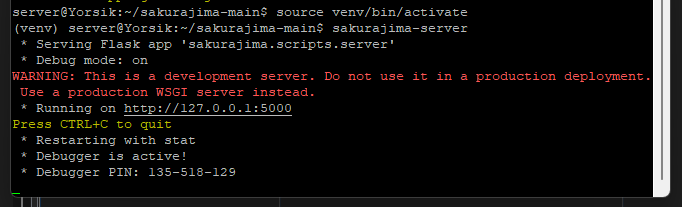
\includegraphics[width=.9\textwidth]{graphics/test/dev_server_run.png}
  \caption{1}
  \label{fig:test1}
\end{figure}

Проведем тестирование заявленного функционала:

\begin{enumerate}

\item Справка по командам


\item Авторизация и аутификация


\item Создание модуля

Чтобы создать модуль, необходимо там, где вы хотите сделать модуль, создать папку с названием данного модуля и в ней же создать файл module.json, где вы должны указать имя модуля и версию модуля. Создадим модуль с названием demo 1.0.0

\begin{figure}
  \centering
  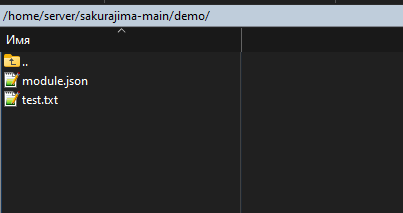
\includegraphics[width=.6\textwidth]{graphics/test/demo_r.png}
  \caption{1}
  \label{fig:test1}
\end{figure}
\newpage
    \item Отправка модуля

После этого, прописываем sakurajima upload demo, что заливает модуль demo на сервер.

\begin{figure}
  \centering
  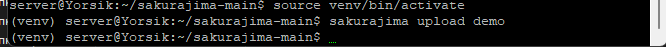
\includegraphics[width=1.0\textwidth]{graphics/test/demo.png}
  \caption{1}
  \label{fig:test1}
\end{figure}

В итоге, на сервере появляется конкретная версия модуля и последняя версия.

\begin{figure}
  \centering
  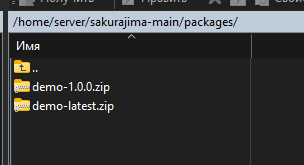
\includegraphics[width=.7\textwidth]{graphics/test/demo_alias_modules.png}
  \caption{1}
  \label{fig:test1}
\end{figure}

\item Обновление модуля

Изменим версию модуля в файле и добавим еще один файл - картинку. Снова выполним команду sakurajima upload demo.

\begin{figure}
  \centering
  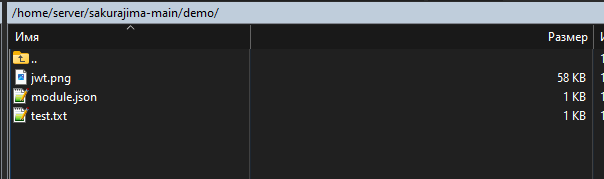
\includegraphics[width=.8\textwidth]{graphics/test/demo_jwt.png}
  \caption{1}
  \label{fig:test1}
\end{figure}

\newpage

Теперь у нас имеется две версии - 1.0.0 и 1.5.0.

\begin{figure}
  \centering
  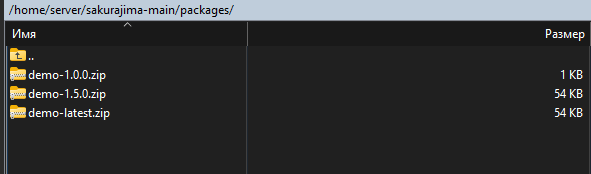
\includegraphics[width=.8\textwidth]{graphics/test/demo_jwt_final.png}
  \caption{1}
  \label{fig:test1}
\end{figure}

\item Загрузка модуля

Проверяем работу скачивания модуля demo, предварительно удалив локально для себя упоминания о нем.

Используем команду: sakurajima install name-module==version

Обычная установка уставливает самую последную версию модуля (latest).
\begin{figure}
  \centering
  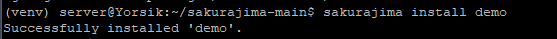
\includegraphics[width=.8\textwidth]{graphics/test/dev_install.png}
  \caption{1}
  \label{fig:test1}
\end{figure}

Если мы укажем через ==версия, то будет загружена определенная версия модуля.

\begin{figure}
  \centering
  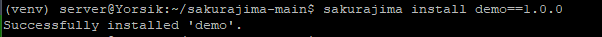
\includegraphics[width=.8\textwidth]{graphics/test/dev_install_ver.png}
  \caption{1}
  \label{fig:test1}
\end{figure}

\newpage

\item Удаление модуля

Используем команду: sakurajima uninstall name-module

\begin{figure}
  \centering
  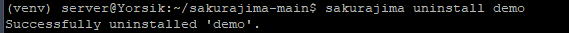
\includegraphics[width=.8\textwidth]{graphics/test/dev_uninstall.png}
  \caption{1}
  \label{fig:test1}
\end{figure}

\item Проверка модуля на увязвимости

Используем команду: sakurajima cve

\item Система зависимостей в модулях

\item Информирование о модуле

Используем команду: sakurajima info


\end{enumerate}

%%% Local Variables:
%%% mode: latex
%%% TeX-master: "rpz"
%%% End:
